\documentclass{report}
\usepackage[utf8]{inputenc}    
\usepackage[T1]{fontenc}
\usepackage[francais]{babel}
\usepackage{wrapfig}
\usepackage{graphicx}
\usepackage{listings,xcolor}
\usepackage{appendix}
\usepackage{adjustbox}
\usepackage{titling}

%Géométrie des pages
\usepackage{geometry}
\geometry{hmargin=2.5cm,vmargin=2.5cm}

%Définition des couleurs pour le code xml
\definecolor{colorxmlnode}{rgb}{0.2, 0.2, 0.2} 
\definecolor{maroon}{RGB}{178 34 34}



%lst xml
\lstdefinelanguage{XML}
{
  basicstyle=\ttfamily,
  morestring=[s]{"}{"},
  morecomment=[s]{?}{?},
  morecomment=[s]{!--}{--},
  commentstyle=\color{darkgreen},
  moredelim=[s][\color{black}]{>}{<},
  moredelim=[s][\color{red}]{\ }{=},
  stringstyle=\color{blue},
  identifierstyle=\color{maroon}
}


\addto\captionsfrench{%
  \renewcommand\appendixname{Annexe}
  \renewcommand\appendixpagename{Annexes}
}

\newcommand\noeud[1]{\textcolor{colorxmlnode}{<\mbox{#1}>}}


\setlength{\droptitle}{-10em}   % This is your set screw


\pretitle{%
  \begin{center}
  \LARGE
  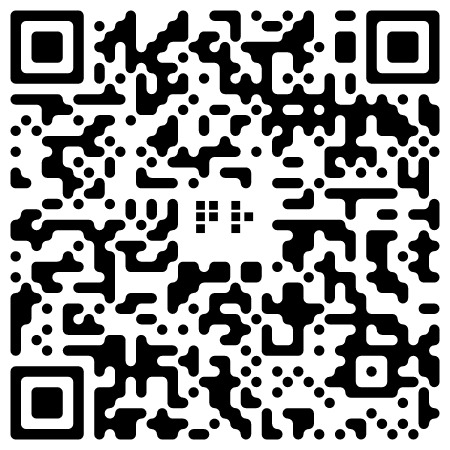
\includegraphics[width=5cm,height=5cm]{img/qr.jpeg}\\[30px]
}
\posttitle{\end{center}}


\title{% 
		Développement d'un couple d'applications bureau et mobile\\ \large
		Génération et lecture de QR Codes pour l'institut Montéclair}
\author{David \bsc{Dembele}\\ Alassane \bsc{Diop}\\
		Jules \bsc{Leguy}\\ Rahmatouwalet \bsc{Mohamedoun}}
\date{Décembre 2017}



\begin{document}

\maketitle

\tableofcontents

\chapter{Introduction}

	\section{Contexte}
		
\par
Dans le cadre du module Concrétisation Disciplinaire de notre première année de Master 1 mention Informatique à l'Université d'Angers, nous avons développé une application de bureau et poursuivi le développement d'une application mobile.

\par
Ces applications répondent à une demande de l'Institut Montéclair à Angers, dans le but d'apporter une dimension ludique à l'enseignement pour les mal-voyants et non-voyants inscrits à l'institut.

\par
Ce projet a été encadré par Corentin \bsc{Talarmain} et Thomas \bsc{Calatayud}, deux étudiants en deuxième année de Master, dans le cadre de leur module Gestion de Projet.\\

\par
L'objectif du projet est de fournir la possibilité aux transcripteurs de l'institut un moyen de générer des QR Codes contenant du texte et des sons et pouvant être interprétés par une application mobile. Une première version de l'application mobile avait déjà été développée par Corentin \bsc{Talarmain} lors de son TER\footnote{Travail Encadré de Recherche} de fin de première année de Master. Celle-ci fournissait déjà la possibilité de lire avec une voix de synthèse du texte contenu dans des QR Codes.
Nous avons donc développé une application de bureau permettant de générer ces QR Codes selon les contraintes décrites dans le cahier des charges. Nous avons également adapté l'application mobile existante à notre nouveau format de données.

	
	\section{Cahier des charges}
		\par
Les transcripteurs souhaitaient néanmoins étendre les fonctionnalités de l'application mobile initiale, qui présentait quelques inconvénients limitant son utilisation. Ne présentant que la possibilité de lire des QR Codes, elle imposait le passage par des sites internet pour en générer. On ne pouvait ainsi pas contrôler la taille maximale des QR Codes générés, parmi lesquels certains étaient trop gros pour être détectables par l'application. En outre, elle ne fournissait pas la possibilité de lire des sons à partir de données contenues dans un QR Code.\\

\par
Les transcripteurs de l'institut nous ont également fourni deux demandes précises autour desquelles nous avons structuré notre projet. La première demande était de pouvoir utiliser les QR Codes comme légendes de cartes de géographie pour des lycéens. Cela implique de pouvoir gérer la lecture de QR Codes adjacents dans un ordre prédéfini, peu importe l'ordre de lecture effectif (LIEN FAMILLES).
\par
L'autre demande était de pouvoir utiliser des QR Codes pour lire des sons dans les pages d'un livre pour enfants, sans avoir nécessairement accès à internet au moment de la lecture. Pour cela, un ou plusieurs QR Codes sur la page de couverture doivent permettre le téléchargement de tous les sons contenus dans le livre (LIEN ENSEMBLE).
\par
En outre, un espace central contenant du texte en braille devait pouvoir être inséré au centre des QR Codes, pour permettre aux non-voyants de les localiser (LIEN GENERATION QR).


\chapter{Organisation}

	\section{Répartition des tâches}
		\input{Organisation/repartitionDesTaches.tex}
	
	\section{Planning}
		\input{Organisation/planning.tex}
		
		
\chapter{Conception}

	\section{Types de QRCodes}
		\par
À partir des contraintes définies dans les cahier des charges (REF CAHIER CHARGES), il a fallu définir précisément quels types de QR Codes allaient être crées. Une première version de notre architecture collait aux besoins de l'Institut Montéclair qui nous ont été transmis. Elle comprenait des QR Codes pour les cartes géographiques, des QR Codes pour les pages d'un livre et des QR Codes pour les pages de couverture des livres. Mais cette architecture s'est avérée trop spécifique et empêchait les transcripteurs de l'institut de créer des QR Codes pour d'autres supports.\\

\par
Nous avons donc créé une seconde version qui respectait les contraintes transmises par l'institut tout en étant la plus généraliste possible, afin d'être utilisable dans tous les contextes compatibles avec les contraintes transmises. Cette architecture est composée de QR Codes contenant un ensemble de textes et de fichiers et pouvant être organisés en familles afin d'être lus dans un ordre prédéfini (les QR Codes atomiques), et de QR Codes contenant un ensemble de liens vers des sons devant être téléchargés sans être joués (les QR Codes ensembles).
		
	\section{Représentation des données}
		\par
Les QR Codes devant stocker plus d'informations que dans la version initiale de l'application mobile, il nous a fallu définir une structure de données pour les représenter. Cette représentation s'est construite parallèlement à l'élaboration des types de QR Codes (LIEN TYPES QR) et à celle du Modèle (LIEN MODÈLE), afin d'assurer la cohérence de l'ensemble.
\par
Notre choix s'est porté sur une structure XML\footnote{Hypertext Markup Language}. Cette structure a montré ses faiblesses par la suite (voir REF CHOIX XML), mais avait déjà crée trop de dépendances pour être modifiée.\\

\par
Afin de minimiser la quantité de données stockées dans le QR Code, seules les données indispensables à l'interprétation du QR Code par l'application mobile y sont stockées. Les données annexes nécessaires au chargement d'un QR Code par l'application de bureau sont stockées dans les métadonnées de l'image (REF CONTROLLEUR/METADONNÉES). On y trouve les données relatives au nom et aux couleurs du QR Code, ou encore au nom des fichiers contenus.
\par
La structure fait apparaître clairement la dichotomie entre les données stockées dans le QR Code (noeud \noeud{donneesUtilisateur}) et les données stockées dans les metadonnées de l'image (noeud \noeud{metadonnees}).\\

\par
Le type de QR Code (atomique ou ensemble) est indiqué par un attribut dans le noeud \noeud{<donneesUtilisateur>}. Ce noeud contient un noeud \noeud{contenu} contenant lui-même un ensemble de textes (\noeud{texte}) et de fichiers (\noeud{fichier}).
\par
L'appartenance à une famille (REF TYPES QR) de QR Codes est indiquée par la présence d'un noeud \noeud{famille} ayant pour attributs le nom de la famille et la place du QR Code.\\

\par
Un exemple complet de représentation XML d'un QR Code est visible dans la figure ci-dessous.

\begin{figure}[!h]
\begin{adjustbox}{minipage=\textwidth,bgcolor={RGB}{240 240 240}}

\lstset{language=XML}

\begin{lstlisting}

<qrcode>
  <donneesutilisateur type="atomique">
    <contenu>
      <texte>champ1</texte>
      <fichier url="URLFICHIER"></fichier>
      <texte>champ2</texte>
    </contenu>
    <famille nom="famille" ordre="4"></famille>
  </donneesutilisateur>
  <metadonnees>
    <fichiers>
      <fichier url="URLFICHIER" nom="fichier1"></fichier>
    </fichiers>
    <colorqrcode color="#085a0c"></colorqrcode>
    <textebraille texte="QR"></textebraille>
    <colorbraille color="#f11313"></colorbraille>
  </metadonnees>
</qrcode>

 
\end{lstlisting}

\end{adjustbox}
\caption{Représentation d'un QR Code}

\end{figure}\textbf{}
		
	\section{Architecture de l'application de bureau}
		\input{Conception/architectureBureau.tex}


\chapter{Réalisation}

	\section{Application de bureau}

		\subsection{Architecture}
			\par
L'application est structurée selon un modèle MVC (Modèle Vue Contrôleur). Les données sont représentées par les classes du modèle, sont traitées par les classes du contrôleur et affichées par la vue. Nous utilisons en outre le patron de conception\footnote{Un patron de conception (souvent appelé design pattern) est un arrangement caractéristique de modules, reconnu comme bonne pratique en réponse à un problème de conception d'un logiciel. Il décrit une solution standard, utilisable dans la conception de différents logiciels. (Wikipédia)} Façade, qui nous permet de limiter la dépendance de la vue au contrôleur à une seule classe. Nous schématisons ces interactions dans la figure suivante.

\begin{figure}[!h]
	\centering
   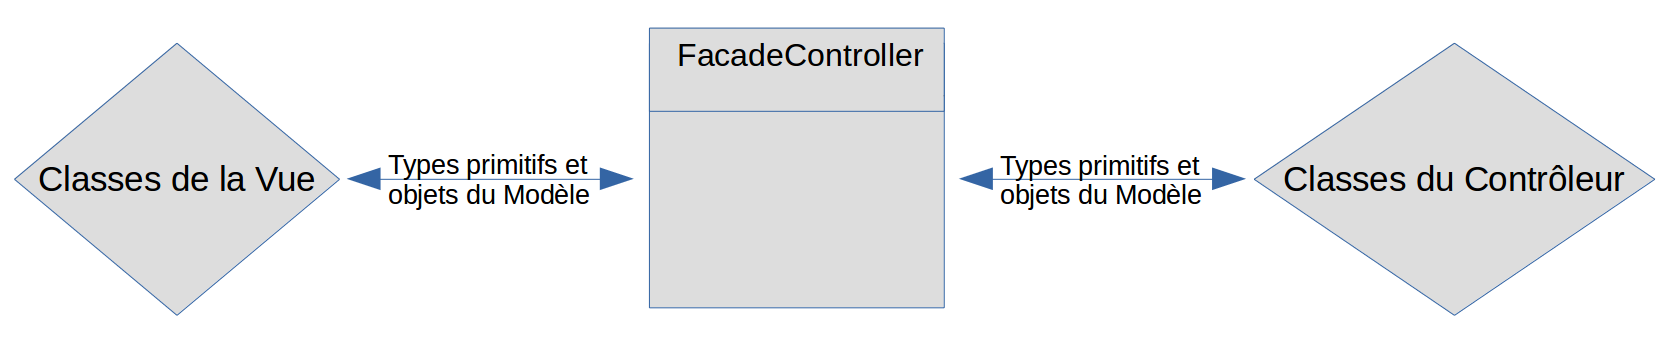
\includegraphics[scale=0.25]{img/facade.png}
   \caption{Interactions entre la vue et le contrôleur à travers la classe FacadeController}
\end{figure}

\par
Le modèle permet de représenter les QR Codes des différents types (voir \ref{typesQR}). Il est composé d'une superclasse abstraite \classe{QRCode}, étendue par deux classes \classe{QRCodeAtomique} et \classe{QRCodeEnsemble} représentant les spécificités des deux types de QR Codes gérés. Le modèle n'effectue pas de traitement des données mais fournit seulement des méthodes permettant d'y accéder et de les modifier, en faisant une abstraction de la façon dont elles sont représentées. Le diagramme UML des classes du modèle est visible ci-dessous.

\begin{figure}[!h]
	\centering
   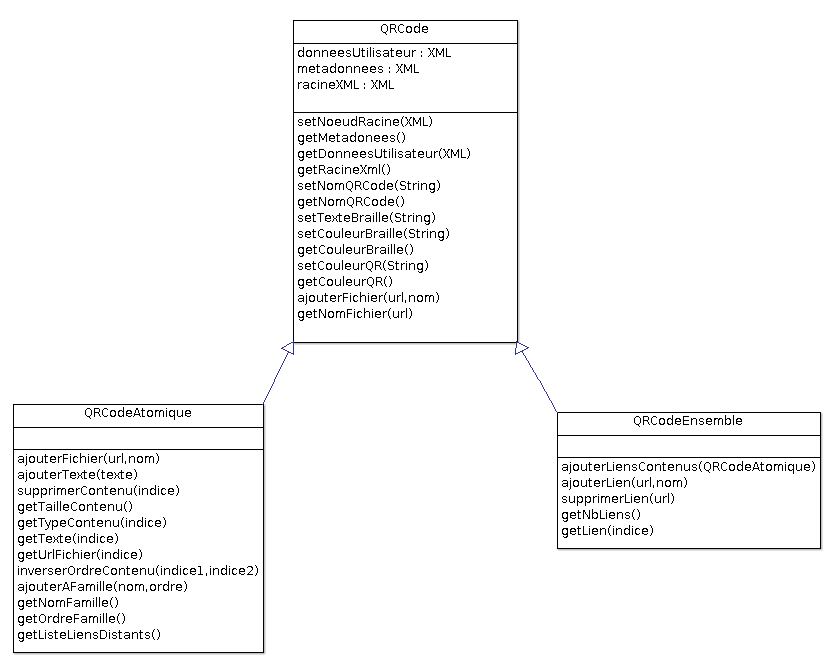
\includegraphics[scale=0.4]{img/modeleUML.png}
   \caption{Diagramme UML des classes du modèle}
\end{figure}

\par
Le contrôleur se charge de tous les traitements permettant de générer des images de QR Codes (voir \ref{generation}), ou d'instancier des objets du modèle à partir d'une image déjà générée (voir \ref{chargement}). L'architecture des classes du contrôleur est visible ci-dessous.


\begin{figure}[!h]
	\centering
   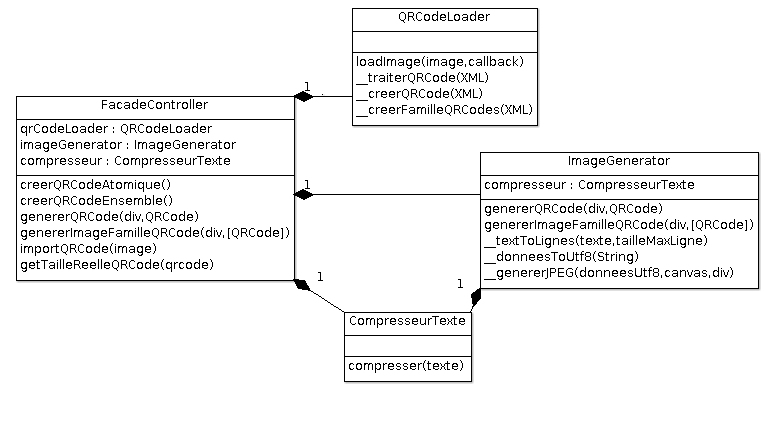
\includegraphics[scale=0.4]{img/controllerUML.png}
   \caption{Diagramme UML des classes du contrôleur}
\end{figure}

\par
La vue est responsable des interactions avec l'utilisateur (voir \ref{interfaceGraphique}). Elle offre une interface permettant de charger, de créer, d'afficher et de gérer des QR Codes.

		\subsection{Modèle}
			\input{Realisation/AppliBureau/modele.tex}

		\subsection{Vue}
			\input{Realisation/AppliBureau/vue.tex}
				
		\subsection{Contrôleur}
			\input{Realisation/AppliBureau/controleur.tex}

	\section{Application mobile}
		
		\subsection{Application existante}
			
\par
Plusieurs fonctionnalités étaient déjà implémentées dans l'application mobile initiale (voir \ref{contexte}). Elle était notamment déjà capable de lire le contenu d'un QR Code via la synthèse vocale de l'API Google text-to-speech et d'interpréter des données structurées en JSON\footnote{JavaScript Object Notation (https://www.json.org)}. En outre, elle offrait déjà la possibilité de lire à la suite plusieurs QR Codes détectés simultanément.

\par
Notre intervention sur l'application a donc consisté à l'adapter aux nouveaux besoins.
Nous avons ainsi modifié certaines parties du code de l’application, notamment ce qui concerne l'interprétation de la structure de données qui est maintenant représentée en XML (voir \ref{representationDonnees} et \ref{compression}).\\

\par
La lecture d’un QR Code se fait donc désormais de la manière suivante. Pour les QR Codes n'appartenant pas à une famille, seul le premier champ est lu (avec la synthèse vocale s'il s'agit d'un texte, ou joué s'il s'agit d'un fichier audio). Il faut effectuer un balayage de l'écran vers la gauche ou la droite pour lire les champs adjacents.
\par
Pour les QR Codes lus simultanément et appartenant à une famille, ils sont lus dans l'ordre spécifié par la famille, tout en permettant toujours le balayage de l'écran pour passer d'un champ à un autre, ou d'un QR Code de la famille à un autre.


		
		\subsection{Adaptation aux nouveaux QR Codes}
			Afin de pouvoir interpréter correctement les QR Codes scannés, nous avons créé un modèle en Java pour l'application Android. Ces classes sont calquées sur les classes du modèle de l'application de bureau (voir \ref{architecture}). Les objets du modèle sont ainsi instanciés à partir des informations lues dans les QR Codes. Ces objets sont ensuite traités pour obtenir le comportement voulu selon chaque type de QR Code scanné.
		
		\subsection{Téléchargement Drive}
			\par
Le téléchargement des fichiers audio s'effectue en utilisant la classe \classe{DownloadManager} d'Android, qui permet de récupérer un fichier distant à partir de son URL\footnote{Uniform Resource Locator (Wikipédia)}. Elle requiert cependant des permissions pour pouvoir stocker les données téléchargées dans l'espace mémoire du téléphone. Seul l'identifiant Google Drive du fichier est stocké dans le QR Code. L'application doit donc recréer l'URL de téléchargement	à partir de cet identifiant. Une fois le fichier téléchargé, il est joué avec la classe \classe{MediaPlayer} d'Android.\\

\par
Une version antérieure de l'application utilisait l'API Google Drive REST pour télécharger les fichiers. Cette version avait pour inconvénient majeur qu'elle forçait la connexion à un compte Google pour télécharger les fichiers, ce qui était peu commode pour les utilisateurs, mais surtout qui posait de graves problème de sécurité pour le compte utilisé. En effet, tous les utilisateurs de l'application obtenaient un accès aux identifiants du compte Google utilisé.
			
	\section{Contraintes et choix}
		\par
Au cours du développement, nous avons dû réaliser un certain nombre de choix techniques. Nous avions parfois plusieurs alternatives et nous avons dû faire des compromis entre complexité de mise en place et efficacité, tout en préservant au mieux la cohérence de l'ensemble.

\par Nous listons ci-dessous les principaux choix effectués ainsi que les raisons qui nous ont poussé à les faire.

\subsection{Langages}

\subsubsection{Développement avec le framework Electron}
\par
Le choix des langages de programmation pour l'application de bureau a été discuté lors de la première séance. Nous avons évoqué le couple Java/Swing qui avait l'avantage d'être le plus simple à programmer mais qui nécessitait un environnement Java sur les machines des utilisateurs. Nous avons également évoqué le couple C++/Qt qui était le plus portable mais potentiellement trop lourd pour l'utilisation qu'on en aurait. 
\par
Les responsables du projet ont finalement opté pour le framework Electron entre les deux premières séances. Ce framework permet de développer des applications de bureau avec des langages web (Javascript/HTML/CSS). Ce choix a été motivé par l'intérêt qu'avait le Javascript d'être facilement utilisable pour accéder à Google Drive (REF STOCKAGE DRIVE).

\subsubsection{Utilisation d'une structure XML et compression}
\par
Nous avons choisi au début du projet d'utiliser une structure XML pour représenter les données stockées dans le QR Code (REF REPR. DONNEES). Ce choix était motivé principalement par la facilité de gestion du XML en JavaScript.
\par
Le XML a toutefois posé des problèmes au niveau de la concision des QR Codes générés. Nous avons tenté de remplacer la structure XML par une structure JSON plus concise lors de la première semaine de décembre, mais nous avions déjà trop de dépendances au XML. Nous avons alors tenté d'utiliser des librairies convertissant le XML déjà généré en JSON avant l'insertion des données dans le QR Code, mais nous n'en avons trouvé aucune suffisamment fiable (les attributs des noeuds xml étaient très mal gérés, et les noeuds de même nom étaient fusionnés sans respecter leur ordre).
\par
Nous nous sommes donc orientés vers une solution de compression pour compenser l'intérêt qu'avait le JSON sur le XML (REF COMPRESSION). Cette solution offre de très bon résultats (toutes les chaînes XML de plus de deux caractères sont compressées en un caractère utf-8 codé sur deux octets). Toutefois, elle ne compresse que la représentation des données et pas les données en elles-mêmes.


\subsection{Technologies et formats}

\subsubsection{Stockage des fichiers distants dans Google Drive}
\par
Le stockage des fichiers sur un serveur distant était indispensable car on ne peut pas stocker des données binaires représentant un fichier mp3 dans un QR Code de taille raisonnable.
Les transcripteurs de l'institut l'utilisant déjà, le drive de Google a été la solution la plus simple. Cette solution présente également l'avantage de ne pas nécessiter la mise en place et la location d'un serveur.


\subsubsection{Connexion à Google Drive dans l'application Android}
\par
L'utilisation de Google Drive a pour principal inconvénient de forcer l'utilisation des API\footnote{Application Programming Interface : Ensemble ce classes, de méthodes et de fonctions. Ici pour accéder aux données stockées sur Google Drive.} de Google. En effet, même pour un fichier disponible publiquement, on ne peut pas le télécharger directement sans passer par un navigateur ou par une des API Google. La commande wget sur l'URL du fichier renvoie la page de téléchargement HTML du fichier et pas le fichier lui-même. Nous aurions peut-être pu récupérer le fichier en analysant la page HTML reçue, mais cela aurait rendu l'application dépendante à la syntaxe de cette page pouvant être modifiée par Google à tout moment.
\par
Pour ces raisons, nous avons été contraints d'implémenter l'API Google Drive REST dans l'application Android, et donc d'imposer une authentification pénible aux utilisateurs.

\subsubsection{Format de sauvegarde des images (JPG)}
\par
Afin de pouvoir insérer des informations dans les métadonnées des images générées par l'application de bureau (REF STRUC DONNEES), nous avons recherché les librairies Javascript permettant de créer une image à partir d'un canvas HTML5 et d'insérer les métadonnées pendant le processus de génération de l'image. Nous n'avons trouvé que des librairies permettant d'insérer des métadonnées de type EXIF\footnote{Exchangeable Image File Format}, qui sont présentes dans les fichiers JPEG mais pas PNG. Il s'agit de la raison pour laquelle nous avons utilisé ce format.



\subsection{Choix d'implémentation}

\subsubsection{Gestion des droits et bouton de connexion dans l'application Android}
\par
Le bouton de connexion au drive de Google (REF CONNEXION DRIVE ANDROID) est né de la volonté de rendre l'application Android utilisable pour lire les QR Codes ne nécessitant pas de connexion au drive sans avoir à se connecter. Cela respecte la philosophie des dernières versions d'Android de ne demander les permissions que lorsqu'elles sont nécessaires.
\par
Les permissions indispensables au fonctionnement de l'application (caméra, vibreur) sont demandées au démarrage de l'application, tandis que la connexion au drive se fait de manière volontaire.
\par
La présence du bouton sur l'écran de détection provient de la complexité de passer des objets complexes entre deux activités sur Android. Il était initialement prévu de placer ce bouton dans l'écran d'options mais cela nous aurait demandé trop de temps à l'approche du délai de fin de projet. Pour laisser tout de même la possibilité de se déconnecter du drive lorsque la connexion est effectuée et que le bouton disparaît dans un souci d'ergonomie, un bouton de déconnexion est présent dans l'activité d'options.



\chapter{Conclusion}
	\par
Tout au long du développement, nous nous sommes efforcés de produire des applications répondant concrètement aux demandes de l'institut Montéclair, tout en gardant à l'esprit que les besoins de l'institut pourraient évoluer. Par conséquent, nos applications ne se veulent pas des versions définitives. En dehors du travail qui reste à effectuer pour les rendre totalement utilisables au quotidien, nous avons tenté de les rendre ouvertes à l'extension pour des versions futures avec peut-être d'autres types de QR Codes, d'autres types de contenus ou d'autres méthodes d'optimisation de la quantité de données contenues dans les QR Codes.\\
Cette volonté s'est traduite par la réalisation d'une architecture des classes souple et non spécifique aux besoins qui nous ont été transmis. Nous avons en outre fait en sorte que la compression des données, qui est la partie la plus susceptible d'être modifiée, soit modulable tout en restant facilement compatible avec les QR Codes que nous générons actuellement.\\

\par
Il reste toutefois une dernière phase de développement avant de pouvoir livrer un couple d'applications totalement fonctionnelles. Les modifications restantes concernent principalement l'interface graphique de l'application de bureau, afin qu'elle soit plus ergonomique avec un système de liste de QR Codes plutôt que d'onglets, un système de glisser-déposer de fichiers provenant de Google Drive, et l'implémentation de la création de QR Codes de type ensemble, permettant de télécharger un ensemble de fichiers audio sans les jouer.
\par
Elles concernent également la complétion de l'interprétation des QR Codes par l'application mobile, afin de gérer dynamiquement le téléchargement de fichiers à la lecture, et l'ajout de messages vocaux à destination de l'utilisateur.\\

\par
Lorsque cette phase de finalisation sera terminée, un nouveau projet pourra débuter à partir de là où nous l'avons laissé, comme nous l'avons fait à partir de l'application mobile initiale. En plus de l'implémentation d'éventuelles nouvelles demandes de l'institut Montéclair, un travail complexe mais intéressant pourra être effectué pour compresser le contenu des QR Codes de manière plus efficace, en compressant le texte contenu dans les QR Codes à partir d'un dictionnaire fixe externe. Une solution de transformation du texte en son directement sur l'application de bureau pourrait également permettre de créer des QR Codes contenant des textes de grande taille.







\end{document}